\documentclass{beamer}
\usetheme[titleformat=smallcaps,block=fill]{metropolis} % numbering=fraction
\IfFileExists{fonts.tex}{\input{fonts.tex}}{} % for small caps @ overleaf

\usepackage{amsmath,amssymb,amsthm,graphicx,multirow}
\usepackage[center]{caption}
\usepackage{subfig}
\usepackage{appendixnumberbeamer,booktabs}

\everymath{\displaystyle}
\newtheorem{proposition}{Proposition}
\newcommand{\E}{\mathop{{}\mathbb{E}}}
\newcommand{\floor}[1]{{\left\lfloor{#1}\right\rfloor}}
\newcommand{\ceil}[1]{{\left\lceil{#1}\right\rceil}}
\DeclareMathOperator*{\vol}{vol}
\DeclareMathOperator*{\Vol}{Vol}
\DeclareMathOperator*{\dist}{dist}

\renewcommand{\appendixname}{{Appendix}} % fix warning
\newcommand{\autotitle}{\secname\ifdefempty{\subsecname}{}{~--- \subsecname}}
\newcommand{\clearsubsecname}{\long\def\subsecname{}}
\newcommand{\vtable}[2][c]{% \vtable[<col align>]{<stuff>}
    \renewcommand{\arraystretch}{0.8}%
    \begin{tabular}[c]{@{}#1@{}}#2\end{tabular}}
\newcommand{\smalldisplayskips}{
    \setlength{\abovedisplayskip}{3pt}
    \setlength{\belowdisplayskip}{3pt}}
%\newcommand{\normaldisplayskips}{
%    \setlength{\abovedisplayskip}{8pt}
%    \setlength{\belowdisplayskip}{8pt}}
%\setbeamerfont{bibliography entry author}{size=\footnotesize}
%\setbeamerfont{bibliography entry title}{size=\footnotesize}
%\setbeamerfont{bibliography entry location}{size=\footnotesize}

%%%%%%%%%%%%%%%%%%%%%%%%%%%%%%%%%%%%%%%%%%%%%%%%%%%%%%%%%%%%%%%%%%%%%%%%%%%%%%%%

\title{Expanders in Power Law Graphs}
\author{Anton Cherniavskyi}
\date{October 22, 2018}
\institute{Simon Fraser University}
\titlegraphic{\hfill
\includegraphics[scale=0.08]{images/sfu_logo}}

%%%%%%%%%%%%%%%%%%%%%%%%%%%%%%%%%%%%%%%%%%%%%%%%%%%%%%%%%%%%%%%%%%%%%%%%%%%%%%%%

\begin{document}

\maketitle

\section{Introduction}
\clearsubsecname

\begin{frame}{\autotitle}
    \textbf{A power law} is a relation of the form $f(x)=ax^b$.

    \textbf{Power-law graphs} have either degrees,
    or the number of vertices with a given degree
    proportional to a power law $x^{-\beta}$, for some constant $\beta\geq0$.
    \begin{figure}
        \centering
        \subfloat{{
            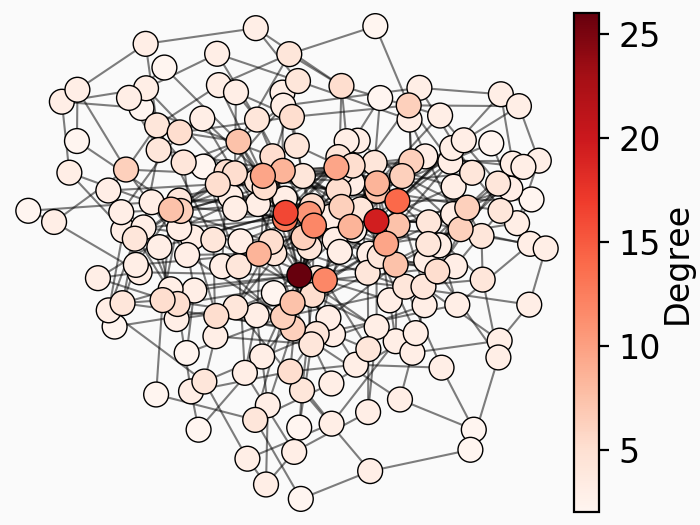
\includegraphics[scale=0.5]
            {images/generated_presentation/power-law-graph}
        }}
        \qquad
        \subfloat{{
            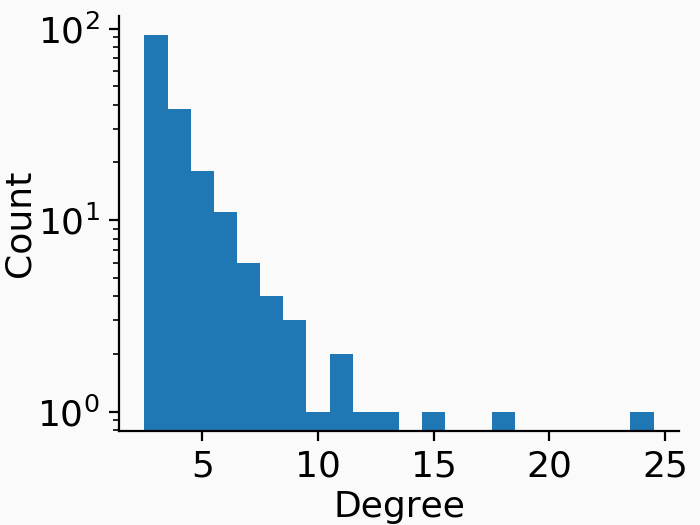
\includegraphics[scale=0.5]
            {images/generated_presentation/power-law-deg-distribution}
        }}
        \caption{Example of a power-law graph and its degree distribution}
    \end{figure}
\end{frame}

\begin{frame}{\autotitle}
    \smalldisplayskips
    \begin{columns}[T,onlytextwidth]
        \column{0.5\textwidth}
        \textbf{$(\alpha n,\gamma)$ edge expander} is a graph
        that for some $\alpha\leq 1/2$ and $\gamma>0$ satisfies:
        \begin{equation*}
            \min_{\substack{S\subset V\\0<|S|\leq\alpha n}}\frac{|\partial S|}{|S|}\geq\gamma
        \end{equation*}
        
        \column{0.5\textwidth}
        \textbf{$(\alpha n,\gamma)$ vertex expander} is a graph
        that for some $\alpha\leq 1/2$ and $\gamma>0$ satisfies:
        \begin{equation*}
            \min_{\substack{S\subset V\\0<|S|\leq\alpha n}}\frac{|N_G(S)|}{|S|}\geq\gamma
        \end{equation*}
    \end{columns}
    ~\\~\\
    
    The size of a cut $(S,V\backslash S)$, for any non-empty $S\subset V$:
    \begin{equation*}
        \partial S=e(S,V\backslash S)=\{(u,v)\in E\;|\;u\in S,v\in V\backslash S\},
    \end{equation*}
    and the external neighborhood of $S$ in $G$:
    \begin{equation*}
        N_G(S)=\{v\in V\backslash S\;|\;\exists u\in S\,((u,v)\in E)\}.
    \end{equation*}
\end{frame}

\begin{frame}{\autotitle}
    \textbf{Motivation:} high expansion means useful expander properties.
    Low expansion indicates a presence of a~sparse cut and
    possible decomposition of a graph.
    
    \textbf{Previous work:} power-law graphs with $2<\beta<3$,
    degrees up to $O\left(\sqrt{n}\right)$ and volume $O(n)$,
    have conductance $\Theta(1)$~by~\cite{gms03}.
    
    \textbf{Methods:} Chernoff bounds for the size of an arbitrary cut,
    generalization of techniques used for regular graphs.
\end{frame}

\subsection{The Main Results}

\begin{frame}{\autotitle}
    \smalldisplayskips
    Coin toss power-law graphs contain $(n'/2,d/2-\delta)$ edge expanders of size
    \begin{equation*}
        n'=
        \begin{cases}
            \Theta(n) & \quad \text{if } \beta\leq 1.6,\\
            \Theta\left(n^{1/\beta}\right) & \quad \text{if } \beta>1.6.
        \end{cases}
    \end{equation*}\\~\\
    
    Permutation power-law graphs have expanders of size $n'=n/2$
    \vspace{-8mm}
    \begin{itemize}
        \item $(n'/2,d/2)$ edge expanders if $\beta\leq 1.72$
        \item $(n'/2,1-\delta)$ and $(\epsilon n',d_0/2-2-\delta)$
        vertex expanders when~$0\leq\beta<1$.
    \end{itemize}

    The diameter of a connected $(\epsilon n,\gamma)$ vertex expander
    is $O(\log n)$ for any constants $0<\epsilon\leq1/2$ and $\gamma>0$.
\end{frame}

\section{Coin Toss Power-Law Graphs}
\clearsubsecname

\begin{frame}{\autotitle}
    \smalldisplayskips
    \textbf{How to generate $G$} given a degree sequence $(w_1,\ldots,w_n)$?
    \begin{equation*}
        \Vol(G)=\sum_{k\in V}{w_k},
        \qquad
        p_{ij}=
        \begin{cases}
            \frac{w_i w_j}{\Vol(G)} & \quad \text{if }i\neq j,\\
            \frac{w_i^2}{2\Vol(G)} & \quad \text{otherwise}.
        \end{cases}
    \end{equation*}
    Edges are independent, degrees are expected.\\~\\
    
    \textbf{The model:} $\E_G[|\{v \in V\;|\;\deg(v)=x\}|]=e^\alpha/x^\beta$,
    where $x\in\{1,\ldots,d_{max}\}$, $d_{max}=e^{\alpha/\beta}$.
    \begin{equation*}
        n=\sum_{x=1}^{e^{\alpha/\beta}}{\frac{e^\alpha}{x^\beta}},
        \qquad \E_G[|E|]=\frac{1}{2}\sum_{x=1}^{e^{\alpha/\beta}}{x\frac{e^\alpha}{x^\beta}}
    \end{equation*}
\end{frame}

\begin{frame}{\autotitle}
    \small
    \begin{theorem}[Existence of an edge expander]
        $\exists d_0\;\forall c<1/3\;\forall\delta>0\;\exists\gamma,c_1=c_1(\beta,c)>0:$
        let $G=(V,E)$ be a random power-law graph from the coin toss model and $H$
        is its induces subgraph of size $n'$ with vertices of degree at least $d_0$.
        
        Then if $0<\beta<1$, the whole graph $G$ is $(n/2,\gamma)$ edge expander w.h.p.
        Otherwise, the subgraph $H$ is $(n'/2,\gamma)$ edge expander w.h.p.
        \begin{equation*}
            n'=
            \begin{cases}
                n & \quad \text{if } 0<\beta<1,\\
                %n/2 & \quad \text{if } \beta=1,\\
                \Theta(n) & \quad \text{if } 1\leq\beta\leq 1.6,\\
                \Theta\left(n^{1/\beta}\right) & \quad \text{if } \beta>1.6.
            \end{cases}
        \end{equation*}
        $H$ has average degree $d=\Theta(n')$ and edge expansion $\gamma=d/2-\delta$.
    \end{theorem}
\end{frame}

\begin{frame}{\autotitle}
    \begin{lemma}[Edge expansion from the average degree]
        $\forall\delta>0\;\exists\gamma:$
        If the expected average degree of $H$ on $n'$ vertices is $d>10\ln n'$,
        then $H$ is $(n'/2,d/2-\delta)$ edge expander w.h.p.
    \end{lemma}
    \begin{block}{Proof.}
        \smalldisplayskips
        For any disjoint $S,T\subset V_H$:
        $\E_G[|e(S,T)|]=\Vol(S)\Vol(T)/\Vol(H)$.
        If $|S|=s\leq n'/2$, then $\Vol(S)=sd=s\frac{\Vol(H)}{n'}$.
        The expectation of a random variable $X_S=|e(S,V_H\backslash S)|$ is
        \begin{equation*}
            \mu=\E_G[X_S]=\Vol(S)(1-s/n'),
            \qquad\frac{d}{2}\leq\frac{\mu}{s}<d
        \end{equation*}
    \end{block}
\end{frame}

\begin{frame}{\autotitle}
    \begin{proof}[Proof (Cont.)]
        \smalldisplayskips
        We use the Chernoff bound for some $\lambda\in(0;1)$: $\gamma s=(1-\lambda)\mu$.
        Note that $\lambda>0$ requires $\gamma<\mu/s$, so $\gamma<d/2$.\\~\\
        
        $\Pr_G[H\text{ is not expanding}]
        \leq\sum_{s=1}^{n'/2}{\binom{n'}{s}\Pr_{G,S}[X_S\leq\gamma s\;|\;|S|=s]}\leq$
        
        $\leq\sum_{s=1}^{n'/2}{\binom{n'}{s}\exp(-\lambda^2\mu/2)}
        \leq\sum_{s=1}^{n'/2}{\exp\left(\left(
            1+\ln n'
            -\frac{d}{4}
            +\gamma
            \right)s\right)}\leq$
        $\leq\sum_{s=1}^{n'/2}{n'^{-(1+\sigma)s}}=o(1)$.

        The last inequality holds for any $\sigma>0$ when $d>10\ln n'$.
    \end{proof}
\end{frame}

\begin{frame}{\autotitle}
    \small\smalldisplayskips
    \begin{lemma}[Size and volume of the subgraph H]
        If $d_0=c\,d_{max}$ for some $0<c<1$, then
        \begin{gather*}
            n'=
            \begin{cases}
                \Theta(n) & \quad \text{if } \beta<1,\\
                \Theta(n/\ln n) & \quad \text{if } \beta=1,\\
                \Theta\left(n\right)^{1/\beta} & \quad \text{if } \beta>1. %o(n)
            \end{cases}\\
            d=\Vol(H)/n'=\Theta(n')
        \end{gather*}
    \end{lemma}

    \begin{lemma}[Linear size subgraph H]
        Case $\beta=1$: if $d_0=d_{max}/\sqrt{n}$, then $n'=n/2$,
        
        Case $\beta>1$: if $d_0=d_{max}/n^{1/\beta}$, then
        $n'\approx\frac{n}{(\beta-1)\,\zeta(\beta)^{1/\beta}}=\Theta(n)$,
        
        $(\beta-1)\,\zeta(\beta)^{1/\beta}>1$ requires $\beta\leq 1.6$,
        in which case $d=\omega(\ln n')$.
    \end{lemma}
\end{frame}

\begin{frame}{\autotitle}
    \begin{proof}[Proof of the main theorem]
        For $1\leq\beta\leq 1.6$, we use lemma about linear size of $H$,
        which gives us $d=\Theta\left(n'^{(2-\beta)/\beta}\right)$ with $n'=\Theta(n)$.

        Otherwise, $d=\Theta(n')$ by more general lemma
        about the size and the volume of $H$.
        For $0<\beta<1$ it is possible to choose $c=0$ thus having $H=G$,
        while the size of $H$ decreases as $n'=\Theta(n^{1/\beta})$ when $\beta>1.6$.
        
        As both of these lemmas guarantee the average degree $d=\omega(\ln n')$,
        $H$ must be $(n'/2,d/2-\delta)$ edge expander.
    \end{proof}
\end{frame}

\section{Permutation Power-Law Graphs}
\clearsubsecname

\begin{frame}{\autotitle}
    \textbf{How to generate $G$} given a degree sequence $(w_1,\ldots,w_n)$?
    
    Randomly permute a sequence with $w_i$ mini-vertices for every $i\in V$,
    and include an edge $(i,j)$ for each consecutive pair of their mini-vertices.
    
    Edges are not independent and degrees are exact.\\~\\
    
    \textbf{The model:} $\deg(v)=w_v=pn/v^\beta,\quad 0<p\leq 1$.
    
    If $\beta=0$, the degree sequence is $(pn,\ldots,pn)$ which is the same
    as the expected degrees of $G(n,p)$ with self-loops.
\end{frame}

\begin{frame}{\autotitle}
    \smalldisplayskips
    $n'=|V_H|$ is the largest number from $\{1,\ldots,n\}$ s.t. $\deg(n')\geq d_0$.
    
    This gives us the size and the volume of $H$:
    \begin{equation*}
        n'\approx(pn/d_0)^{1/\beta},
        \qquad\vol(H)=\sum_{v=1}^{n'}{\frac{pn}{v^\beta}}=d_0n'^\beta H_{n',\beta}
    \end{equation*}
    
    \begin{proposition}[The Sum of a Special Series]
        $S_n=\sum_{s=1}^{\alpha n}{\left(c_1(s/n)^{c_2}\right)^s}$,
        where $0<\alpha\leq 1/2$, $c_1>0$, and $c_2>0$.
        \begin{enumerate}
            \item $S_n\leq o(1)$, for some sufficiently small $\alpha$.
            \item $S_n\leq o(1)$, for $\alpha\leq 1/2$, if $c_2>\max\{1,\log c_1\}$,
            $c_1=o\left(n^{c_2-1}\right)$.
        \end{enumerate}
    \end{proposition}
\end{frame}

\begin{frame}{\autotitle}
    Generalized harmonic numbers:
    \begin{equation*}
        H_{n,\beta}=\sum_{k=1}^{n}\frac{1}{k^\beta}\approx
        \begin{cases}
            \frac{n^{1-\beta}}{1-\beta} & \quad \text{if } \beta<1,\\
            \ln n & \quad \text{if } \beta=1,\\
            \zeta(\beta) & \quad \text{if } \beta>1.
        \end{cases}
    \end{equation*}
    
    Riemann zeta function, defined for $s>1$:
    \begin{equation*}
        \zeta(s)=\sum_{k=1}^{\infty}\frac{1}{k^s}
    \end{equation*}
    For large $x\in\mathbb{R}$: $\zeta(x)\approx 1+2^{-x}$,
    and $\lim_{x\to\infty}\zeta(x)=1$.
\end{frame}

\begin{frame}{\autotitle}
    \begin{theorem}[Existence of an edge expander]
        $\forall 0<p\leq 1\;\exists d_0=d_0(p,n,\beta)\;\forall\delta>0\;\exists\gamma,\epsilon>0:$
        let $G$ be a random power-law graph with $\deg(v)=pnv^{-\beta}$,
        and $H$ is its induced subgraph of size $n'$ obtained by retaining vertices of degree at least $d_0$.
        
        Then if $\beta=0$, the whole graph $G$ is $(\epsilon n,\gamma)$ edge expander w.h.p.
        Otherwise, $H$ is $(\epsilon n',\gamma)$ edge expander w.h.p.
        
        When $\beta>1$, the additional requirement is $p\,\zeta(\beta)>2$.
        More~roughly, $\zeta(\beta)>2$ and $\beta\leq 1.72$.
    \end{theorem}
\end{frame}

\begin{frame}{\autotitle}
    \begin{theorem}[Cont.]
        \smalldisplayskips
        If $\beta=0$: $d_0=pn, \qquad\quad\;\, n'=n, \quad\;\;\;\,\gamma=d-2-\delta$.\\
        If $\beta>0$: $d_0=2^\beta pn^{1-\beta}, \quad n'=n/2, \quad\gamma=d/2$.

        The average degree of $H$:
        \begin{equation*}
            d=
            \begin{cases}
                pn & \quad \text{if } \beta=0,\\
                \Theta(n^{1-\beta}) & \quad \text{if } 0<\beta<1,\\
                \Theta(\ln n) & \quad \text{if } \beta=1,\\
                2p\,\zeta(\beta)=\Theta(1) & \quad \text{if } \beta>1.
            \end{cases}
        \end{equation*}
    \end{theorem}
\end{frame}

\begin{frame}{\autotitle}
    \smalldisplayskips
    \begin{block}{Proof.}
        Case $\beta=0$: $\deg(v)=pn$ for each $v\in V$, so we choose $d_0=pn$.
        Then~trivially $H=G$ and the proof is reduced to known case for regular graphs.
        When $\beta>0$, we generalize that approach.
        
        We want a linear size $H$:
        \begin{gather*}
            n'=(pn/d_0)^{1/\beta}=n/2\\
            d_0=2^\beta pn^{1-\beta}=2pn'^{1-\beta}\\
            d=\vol(H)/n'
        \end{gather*}
    \end{block}
\end{frame}

\begin{frame}{\autotitle}
    \small
    \begin{block}{Proof (Cont.)}
        $\Pr_G[H\text{ is not expanding}]
        =\sum_{s=1}^{\epsilon n'}{
            \binom{n'}{s}
            \Pr_{G,S}[|e(S,V_H\backslash S)| < \gamma s]
        }=$
        $=\sum_{s=1}^{\epsilon n'}{
            \binom{n'}{s}
            \Pr_{G,S}\left[|e(S,S)|\geq\frac{\vol(S)-\gamma s}{2}\right]
        }\leq$
        $\leq\sum_{s=1}^{\epsilon n'}{
            \binom{n'}{s}
            \frac{\binom{\vol(H)/2}{(\vol(S)-\gamma s)/2}\binom{\vol(H)-(\vol(S)-\gamma s)}{\gamma s}}{\binom{\vol(H)}{\vol(S)}}
        }\leq$
        $\leq\sum_{s=1}^{\epsilon n'}{\left(
            \frac{e^{1+\gamma/2}}{\gamma^\gamma}
            e^{d/2}
            \frac{d^{(d+\gamma)/2}}{(d-\gamma)^{(d-\gamma)/2}}
            \left(\frac{s}{n'}\right)^{d/2-\gamma/2-1}
        \right)^s}$.

        At this point we require $d/2-\gamma/2-1>0$, or $\gamma<d-2$.
        
        Let $\gamma=d/2$ so we can simplify further.
    \end{block}
\end{frame}

\begin{frame}{\autotitle}
    \small
    \begin{proof}[Proof (Cont.)]
        $\Pr_G[H\text{ is not expanding}]
        \leq\sum_{s=1}^{\epsilon n'}{\left(
            e
            (2e)^{3d/4}
            \left(\frac{s}{n'}\right)^{d/4-1}
        \right)^s}$.
    \begin{equation*}
        d=
        \begin{cases}
            pn & \quad \text{if } \beta=0,\\
            \frac{2^\beta p}{1-\beta}n^{1-\beta} & \quad \text{if } 0<\beta<1,\\
            2p\ln(n/2) & \quad \text{if } \beta=1,\\
            2p\,\zeta(\beta) & \quad \text{if } \beta>1.
        \end{cases}
    \end{equation*}
    Note that when $\beta>1$, we need $p\,\zeta(\beta)>2$.
    
    Finally, we consider small and large values of $s$ separately to get:
    
    $\Pr_G[H\text{ is not expanding}]=o(1)$.
    \end{proof}
\end{frame}

\begin{frame}{\autotitle}
    \smalldisplayskips
    \begin{theorem}[Existence of a vertex expander]
        $\forall 0<p\leq 1\;\exists d_0=d_0(p,n,\beta)\;\forall\delta>0\;\exists\gamma,\epsilon>0:$
        let $G$ be a random power-law graph from the permutation model with $\deg(v)=pnv^{-\beta}$,
        and $H$ is its induced subgraph of size $n'$ obtained by retaining vertices of degree at least $d_0$.
        
        Then if $\beta=0$, $G$ is $(\epsilon n,\gamma)$ vertex expander w.h.p.\\
        Else $0<\beta<1$ and $H$ is $(\epsilon n',\gamma)$ vertex expander w.h.p.

        Either $\epsilon=1/2$ and $\gamma=1-\delta$,
        or $\epsilon$ is sufficiently small and
        \begin{equation*}
            \gamma=\begin{cases}
                d/2-2-\delta & \quad \text{if } \beta=0,\\
                d_0/2-2-\delta & \quad \text{if } 0<\beta<1,
            \end{cases}
        \end{equation*}
    \end{theorem}
\end{frame}

\begin{frame}{\autotitle}
    \begin{block}{Proof.}
        Case $\beta=0$: $G$ is $pn$-regular graph, and the original proof
        with our proposition about the sum of a special series suffice.
        Otherwise, $\beta>0$: proceed like for $d$-regular graphs,
        but instead of $d$ perfect matchings on $n$ vertices
        we have one perfect matching on $\vol(H)$ mini-vertices.
        
        For any $S\subset V_H$ of size $s\leq\epsilon n'$
        and any $T\subset V_H$ of size $(1+\gamma)s$:
        \begin{equation*}
            d=\frac{\vol(H)}{n'},
            \qquad\vol(S)=sd,
            \qquad\vol(T)=(1+\gamma)sd
        \end{equation*}
    \end{block}
\end{frame}

\begin{frame}{\autotitle}
    \smalldisplayskips
    \begin{block}{Proof (Cont.)}
        All mini-vertices from $S$ are matched to mini-vertices in $T$ with probability:
        $\Pr_{G,S,T}[N_H(S)\subseteq T]\leq\left(\frac{\vol(T)}{\vol(H)}\right)^{\vol(S)/2}$.

        The number of sets $S$ is $N_S=\binom{\vol(H)/d_0}{\vol(S)/d_0}$.

        $\Pr_G[H\text{ is not expanding}]
        \leq\sum_{s=1}^{\epsilon n'}{
            N_S
            N_T
            \left(\frac{\vol(T)}{\vol(H)}\right)^{\vol(S)/2}\leq
        }$
        $\leq\left(
            e^{(2+\gamma)d/d_0}
            (1+\gamma)^{d(1/2-(1+\gamma)/d_0)}
            \left(\frac{s}{n'}\right)^{d(1/2-(2+\gamma)/d_0)}
        \right)^s$.
    \end{block}
\end{frame}

\begin{frame}{\autotitle}
    \smalldisplayskips
    \begin{proof}[Proof (Cont.)]
        The exponent of $s/n'$ is positive if $0\leq\gamma<d_0/2-2$, $d_0>4$.
        
        When $\beta>0$, this condition turns into:
        \begin{equation*}
            d_0=2^\beta pn^{1-\beta}>4,
            \qquad n^{1-\beta}>2^{2-\beta},
            \qquad\beta<1
        \end{equation*}
        By the proposition about the sum of a special series:
        $\Pr_G[H\text{ is not expanding}]=o(1)$,
        
        when either $\epsilon$ is a small constant,
        or $\epsilon=1/2$ but $\gamma<1$ in~order to satisfy $c_2>\log c_1$.
    \end{proof}
\end{frame}

\section{Diameter of Vertex Expanders}
\clearsubsecname

\begin{frame}{\autotitle}
    We focus on $(\epsilon n,\gamma)$ vertex expanders,
    especially when $\epsilon<1/2$.
    \begin{block}{Example (Connectivity)}
        A graph $G$ consists of two disconnected $(n/4,\gamma)$
        vertex expanders of size $n/2$ each.
        Any subset of $G$ of size up to $n/4$ is the union of subsets
        of these two parts, and it expands proportionally.
        Therefore, $G$ is $(n/4,\gamma)$ vertex expander too.
    \end{block}
    \begin{theorem}[\cite{hlw06}]
        $(n/2,\gamma)$ vertex expanders have diameter $O(\log n)$.
    \end{theorem}
\end{frame}

\begin{frame}{\autotitle}
    \begin{theorem}[Diameter of vertex expanders]
        Let $G=(V,E)$ be connected $(s(n),\gamma)$ vertex expander of size $n$,
        where $s(n)\leq n/2$ and $\gamma=\Omega(1)$.
        
        Then the diameter of $G$ is $O\left(\frac{n}{s(n)}\log s(n)\right)$.
    \end{theorem}
    \begin{corollary}
        The diameter of a connected $(\epsilon n,\gamma)$ vertex expander of size $n$,
        where $\epsilon\leq1/2$ and $\gamma$ are some positive constants, is $O(\log n)$.
    \end{corollary}
\end{frame}

\begin{frame}{\autotitle}
    \small\smalldisplayskips
    \begin{lemma}[Partitioning of vertex expanders]
        If $G=(V,E)$ is $(s(n),\gamma)$ vertex expander,
        there exists a partitioning $\{S_1,\ldots,S_k\}$ of $V$,
        $k=O\left(\frac{n}{s(n)}\right)$ and $S_i$ has diameter $O(\log s(n))$.
    \end{lemma}

    \begin{proof}
        Let $B(v,r)=\{u\in V\;|\;\dist(v,u)\leq r\}$, then for any $v\in V$ and $r\geq 1$:
        \begin{equation*}
            |B(v,r-1)|\leq s(n)\implies
            |B(v,r)|\geq\min\left\{s(n),(1+\gamma)^r\right\}
        \end{equation*}
        There is $r_0=\ceil{\log_{1+\gamma}s(n)}=\Theta(\log s(n))$
        such that $|B(v,r_0)|\geq s(n)$.
        
        Pick arbitrary $v_1\in V$ and select $S_1=B(v_1,r_0)$.
        Repeat until $B(v_i,r_0)$ contains less than $s(n)/2$ of not selected vertices.
        We stop after $k\leq2n/s(n)$ steps, every remaining vertex
        is within distance $r_0$ from some $S_j$, 
        so we add each of them to the corresponding $S_j$.
    \end{proof}
\end{frame}

\begin{frame}{\autotitle}
    \begin{proof}[Proof of the theorem.]
        The lemma gives us the partitioning $\{S_1,\ldots,S_k\}$ of $V$.
        
        Create a graph $G'$ of size $k$ from $G$ by contracting each $S_i$
        into a single vertex and merging multiple edges.
        Note that $G'$ is connected by construction.
        
        For any $u,v$ from $G$, the distance between
        their corresponding vertices in $G'$ is at most $k$.
        Let $D$ be the maximum diameter of any $S_i$.
        Then $\dist(u,v)$ in $G$ is at most $k(2D+1)$
        which equals $O\left(\frac{n}{s(n)}\log s(n)\right)$.
    \end{proof}
\end{frame}

\section[Comparison of the Results]{Comparison}
\clearsubsecname

\begin{frame}{\autotitle}
    \small
    \begin{table}
        \caption{Power-law graph models}
        \begin{tabular}{@{} lll @{}}
            \toprule
            Model & Object & Definition\\
            \midrule
            Model from~\cite{acl01} & \vtable[l]{exact\\frequencies}
                & $|\{i \in V\;|\;\deg(i)=x\}|=\frac{e^\alpha}{x^\beta}$\\[10pt]
            \textbf{Coin toss model} & \vtable[l]{expected\\frequencies}
                & $\E_G[|\{i\in V\;|\;\deg(i)=x\}|]=\frac{e^\alpha}{x^\beta}$\\[10pt]
            \vtable[l]{The ``octopus'' graphs\\from~\cite{cl04}} & \vtable[l]{expected\\degrees}
                & $\E_G[\deg(i)]=ci^{-1/(\beta-1)}$\\[10pt]
            \textbf{Permutation model} & \vtable[l]{exact\\degrees}
                & $\deg(i)=\frac{pn}{i^\beta}$\\
            \bottomrule
        \end{tabular}
    \end{table}
\end{frame}

\subsection{Random \texorpdfstring{$d$}{d}-regular Graphs}

\begin{frame}{\autotitle}
        \begin{theorem}[\cite{hlw06}]
        $\forall d\geq3\;\forall \delta>0\;\exists\gamma,\alpha>0:$
        a random $d$-regular graph on $n$ vertices is
        $(\alpha n,\gamma)$ edge expander and $(\alpha n,\gamma)$ vertex expander w.h.p.
        with $\gamma=d-2-\delta$.
    \end{theorem}
    
    \begin{theorem}[\cite{bol88}]
        $\forall d\geq3\;\forall 0<\epsilon<1:$ if
        $(1-\epsilon)^{(1-\epsilon)}(1+\epsilon)^{(1+\epsilon)}>2^{4/d}$,
        then any random $d$-regular graph $G$ has $h(G)\geq\gamma=(1-\epsilon)d/2$ w.h.p.
    \end{theorem}

    \textbf{The Cheeger constant}: $h(G)\geq\gamma$ in $(n/2,\gamma)$ edge expander.\\
    The infinite $d$-regular tree has $h(T)=d-2+o(1)$,\\
    and random $d$-regular graphs have $h(G)\leq d/2+o(1)$.
\end{frame}

\subsection{Uniform Random Graphs}

\begin{frame}{\autotitle}
    \begin{description}
        \item[$G(n,p)$] is a graph with $\Pr_G[(i,j)\in E]=p$, for any $i,j\in V$.
        \item[$G(n,m)$] is a graph with exactly $m$ edges,
        and each of $\binom{N}{m}$ graphs is chosen uniformly at random.
    \end{description}
    $N=\binom{n}{2}$ is the maximum number of edges in a simple graph.
    
    If $m=pN$ and $p>\frac{\log n}{n}$ as $n\to\infty$,
    then $G(n,p)$ and $G(n,m)$ are almost identical.
\end{frame}

\begin{frame}{\autotitle}
    \begin{theorem}[Expanders in ``locally-sparse'' graphs \cite{kri17}]
        $\forall c_1>c_2>0\;\forall 0<\alpha<1\;\forall\Delta>0\;\exists\gamma>0:$
        if $G=(V,E)$ has degree $\Delta(G)\leq\Delta$ and $\frac{|E|}{|V|}\geq c_1$,
        then either some $W\subset V$ of size $|W|\leq\alpha n$ spans at least $c_2|W|$ edges,
        or there is an induced $(|W|/2,\gamma)$ vertex expander on $|W|\geq\alpha n$ vertices.
    \end{theorem}
    
    \begin{corollary}[Expanders in $G(n,p)$ \cite{kri17}]
        $\forall\epsilon>0\;\exists\gamma>0:$ a random graph $G\left(n,\frac{1+\epsilon}{n}\right)$
        contains w.h.p. an induced bounded degree $(n'/2,\gamma)$ vertex expander
        on $n'\geq\gamma n$ vertices.
    \end{corollary}
\end{frame}

\begin{frame}{\autotitle}
    \begin{columns}[T,onlytextwidth]
        \column{0.5\textwidth}
        $G(n,p)$ becomes connected when $d\approx pn>(1+\epsilon)\log n$.\\~\\~\\~\\~\\
        
        If $p>(1+\epsilon)/n$, $G(n,p)$ contains $(n'/2,\gamma)$ vertex expander
        of size $n'=\Theta(n)$, $\gamma<1$ for $\epsilon<0.89$.
        
        \column{0.5\textwidth}
        By our lemma, the expected average degree $d>10\log n$
        implies $(n/2,d/2-\delta)$ edge expansion.\\~\\~\\
        
        We showed existence of $(n''/2,1-\delta)$ vertex expander
        for the permutation model with $0<\beta<1$, $n''=n/2$.
    \end{columns}
\end{frame}

\subsection{Sizes of Expanders and Connected Components}

\begin{frame}{\autotitle}
    \footnotesize
    \begin{table}
        \caption{Consistency of sizes between different results}
        \begin{tabular}{@{} l|c|c|c|c @{}}
            \specialrule{\heavyrulewidth}{0pt}{0pt}
            & \multicolumn{4}{c}{$\beta$}\rule{0pt}{13pt}\\[3pt]
            \cline{2-5}
            & $(0;1.6]$ & $(1.6;1.72]$ & $(1.72;3.48)$ & $(3.48;\infty)$\rule{0pt}{13pt}\\[3pt]
            \hline
            \vtable[l]{The largest components\\in graphs from~\cite{acl01}}
                & \multicolumn{3}{|c|}{the giant component, $\Theta(n)$}
                & $O\left(n^{2/\beta}\log n\right)$\rule{0pt}{17pt}\\[7pt]
            \hline
            \vtable[l]{Our edge expanders\\in coin toss model}
                & $\Theta(n)$
                & \multicolumn{3}{|c}{$\Theta\left(n^{1/\beta}\right)$}\rule{0pt}{17pt}\\[7pt]
            \hline
            \vtable[l]{Vertex \& edge expanders\\in $G(n,p)$ by~\cite{kri17}}
                & \multicolumn{4}{|c}{$\Theta(n)$}\rule{0pt}{17pt}\\[7pt]
            \hline
            \vtable[l]{Our edge expanders\\in permutation model}
                & \multicolumn{2}{|c|}{$\Theta(n)$}
                & \multicolumn{2}{|c}{---}\rule{0pt}{17pt}\\[7pt]
            \specialrule{\heavyrulewidth}{0pt}{0pt}
        \end{tabular}
    \end{table}
\end{frame}

\section{Conclusions}
\clearsubsecname

\begin{frame}{\autotitle}
    \small
    We have achieved these goals:
    \begin{itemize}
        \item established existence of expanders in power-law graphs under several models
        \item studied their behavior for different ranges of the exponent $\beta$
        \item made an overview and comparison to the results about regular and uniform random graphs:
        \begin{itemize}
            \item power-law graphs with small $\beta$
            have similar to $G(n,p)$ expansion properties
            \item the largest components of power-law graphs have size comparable
            to the size of our edge expanders
        \end{itemize}
    \end{itemize}
\end{frame}

\begin{frame}{\autotitle}
    \small
    Promising directions for future research include:
    \begin{itemize}
        \item tightening gaps between sizes of connected components and expanding subgraphs
        \item developing improved SAT algorithms for power-law formulas
        \item connecting spectral and combinatorial expansion for power-law graphs
        \item improving the quality of expansion:
        \begin{itemize}
            \item extending the range of parameters to have expanding sets
            of size up to $n/2$ instead of just the small ones
        \end{itemize}
        \item studying the expansion of powers $G^k$ of power-law graphs,
        for~some small constant $k$.
    \end{itemize}
\end{frame}

\appendix
\addtocounter{part}{-1} % fix ToC links

\begin{frame}[allowframebreaks]{References}
    \bibliographystyle{alpha}
    \bibliography{references}
\end{frame}

\begin{frame}[standout]
    \centering
    \textbf{The end}
\end{frame}

\section{Notes}
\clearsubsecname

\begin{frame}{\autotitle}
    We work with an induced subgraph $H=(V_H,E_H)$ of $G$,
    obtained~by retaining only vertices of degree at least $d_0$.
    
    $H$ has size $|V_H|=n'$ and the average degree $d=\Vol(H)/n'$.
\end{frame}

\subsection{Conductance of Random Graphs}

\begin{frame}{\autotitle}
    \textbf{The conductance} generalizes the notion of edge expansion:
    \begin{equation*}
        \Phi(G)=\min_{\substack{S\subset V\\0<\vol(S)\leq \vol(G)/2}}
        \frac{|\partial S|}{\vol(S)}
    \end{equation*}
    \begin{theorem}[Conductance of graphs with given degrees~\cite{gms03}]
        If $G=(V,E)$ is a random graph generated according to
        the~permutation model with minimum degree $3$, then w.h.p.
        \begin{equation*}
            \Phi(G)\geq\gamma=0.0175
        \end{equation*}
    \end{theorem}
\end{frame}

\subsection{Properties of Graphs from~\texorpdfstring{\cite{acl01}}{[ACL01]}}

\begin{frame}{\autotitle}
    \small
    \begin{table}
        \caption{Properties of power-law graphs from~\cite{acl01}, $\beta_0\approx3.4785$}
        \begin{tabular}{@{} l|c|c|c|c|c|c @{}}
            \specialrule{\heavyrulewidth}{0pt}{0pt}
                & \multicolumn{6}{c}{$\beta$}\rule{0pt}{13pt}\\[3pt]
            \cline{2-7}
            & $(0;1)$ & $1$ & $(1;2)$ & $2$ & $(2;\beta_0)$ & $(\beta_0;\infty)$\rule{0pt}{13pt}\\[3pt]
            \hline
            \vtable[l]{The largest\\component}
                & $n$ & \multicolumn{4}{|c|}{$\Theta(n)$}
                & $O\left(n^{2/\beta}\log n\right)$\rule{0pt}{17pt}\\[7pt]
            \hline
            $|V|=n$
                & $\frac{e^{\alpha/\beta}}{1-\beta}$ & $\alpha e^\alpha$
                & \multicolumn{4}{|c}{$\zeta(\beta)e^\alpha$}\rule{0pt}{17pt}\\[7pt]
            \hline
            $|E|$
                & \multicolumn{3}{|c|}{$\frac{1}{2}\frac{e^{2\alpha/\beta}}{2-\beta}$}
                & $\frac{1}{4}\alpha e^\alpha$
                & \multicolumn{2}{|c}{$\frac{1}{2}\zeta(\beta-1)e^\alpha$}\rule{0pt}{17pt}\\[7pt]
            \specialrule{\heavyrulewidth}{0pt}{0pt}
        \end{tabular}
    \end{table}
\end{frame}

\subsection{Behavior of \texorpdfstring{$G(n,p)$}{G(n,p)} Graphs}

\begin{frame}{\autotitle}
    \begin{table}
        \caption{The behavior of $G(n,p)$}
        \begin{tabular}{@{} llr @{}}
            \toprule
            \multicolumn{2}{@{} l}{Regime} & Property\\
            \midrule
            \multicolumn{2}{@{} l}{$p=o(1/n)$} & the graph is a disjoint union of trees\\[5pt]
                & $c<1$ & the largest component is $O(\log n)$\\
            $p=c/n$ & $c=1$ & the largest component is $\Theta\left(n^{2/3}\right)$\\
                & $c>1$ & a unique giant component of size $\Theta(n)$\\[5pt]
            \multicolumn{2}{@{}l}{$p<(1-\epsilon)\log n/n$} & the graph is disconnected w.h.p.\\
            \multicolumn{2}{@{}l}{$p>(1+\epsilon)\log n/n$} & the graph is connected w.h.p.\\
            \bottomrule
        \end{tabular}
    \end{table}
\end{frame}

\subsection{Smaller Volume of \texorpdfstring{$H$}{H}}

\begin{frame}{\autotitle}
    \small\smalldisplayskips
    \textbf{Coin toss model:} considering $H$ independently from $G\backslash H$,
    we need to account for $e(H,G\backslash H)$,
    \begin{gather*}
        \Vol(G)=\begin{cases}
            \Theta\left(n^2\right) & \quad \text{if } \beta<1,\\
            \Theta\left(\left(\frac{n}{\log n}\right)^2\right) & \quad \text{if } \beta=1,\\
            \Theta\left(n^{2/\beta}\right) & \quad \text{if } 1<\beta<2,\\
            \Theta\left(n\log n\right) & \quad \text{if } \beta=2,\\
            \Theta\left(n\right) & \quad \text{if } \beta>2.
        \end{cases}\\
            \Vol(H)=\sum_{v\in H}{w_v}=\Theta\left(n'^2\right)=\begin{cases}
            \Theta\left(n^2\right) & \quad \text{if } \beta<1,\\
            \Theta\left(\left(\frac{n}{\log n}\right)^2\right) & \quad \text{if } \beta=1,\\
            \Theta\left(n^{2/\beta}\right) & \quad \text{if } \beta>1.
        \end{cases}
    \end{gather*}
\end{frame}

\begin{frame}{\autotitle}
    \begin{gather*}
        2\,|e(H)|=\Vol(H)-|e(H,G\backslash H)|\\
        |e(H,G\backslash H)|=\frac{\Vol(H)\Vol(G\backslash H)}{\Vol(G)}\\
        |e(H)|=\frac{\Vol(H)^2}{2\Vol(G)}
    \end{gather*}
    \begin{equation*}
        \begin{split}
            |e(G)|=&|e(H)|+|e(H,G\backslash H)|+|e(G\backslash H)|=\\
            =&\frac{\Vol(H)^2/2+\Vol(H)\Vol(G\backslash H)+\Vol(G\backslash H)^2/2}{\Vol(G)}=\\
            =&\frac{(\Vol(H)+\Vol(G\backslash H))^2}{2\Vol(G)}
            =\frac{\Vol(G)^2}{2\Vol(G)}=\frac{\Vol(G)}{2}
        \end{split}
    \end{equation*}
\end{frame}

\begin{frame}{\autotitle}
    How much smaller would $2\,e(H)$ be than $\Vol(H)$ that we use?
    \begin{gather*}
        2\,e(H)=\frac{\Vol(H)^2}{\Vol(G)}=\Vol(H)\,x\\
        x=\frac{\Vol(H)}{\Vol(G)}=
        \begin{cases}
            \Theta(1) & \quad \text{if } \beta<2,\\
            \frac{1}{\log n} & \quad \text{if } \beta=2,\\
            \frac{1}{n^{1-2/\beta}} & \quad \text{if } \beta>2.
        \end{cases}
    \end{gather*}
\end{frame}

\subsection{Error from Rounding Degrees}

\begin{frame}{\autotitle}
    \textbf{Permutation model:} $\deg(v)=\floor{pn/v^\beta}$.
    
    Error of $\vol(G)$ is at most $n$, which is negligible when $0\leq\beta\leq 1$,
    \begin{equation*}
        \vol(H)=
        \begin{cases}
            \Theta\left(n^2\right) & \quad \text{if } \beta=0,\\
            \Theta\left(n^{2-\beta}\right) & \quad \text{if } 0<\beta<1,\\
            \Theta(n \log n) & \quad \text{if } \beta=1,\\
            \Theta(n) & \quad \text{if } \beta>1.
        \end{cases}
    \end{equation*}
\end{frame}

\subsection{\texorpdfstring{``Octopus''}{"Octopus"} Power-Law Graphs}

\begin{frame}{\autotitle}
    \textbf{The ``octopus'' graphs} from~\cite{cl04} have expected degrees
    proportional to a power law, $d$ and $d_{max}$ are parameters:
    \begin{equation*}
        \E_G[\deg(i)]=w_i=ci^{-1/(\beta-1)}
    \end{equation*}
    The graphs are generated according to the coin toss model.
    $i_0\leq i<n+i_0
    \qquad c=\frac{\beta-2}{\beta-1}dn^{\frac{1}{\beta-1}}
    \qquad i_0=n\left(\frac{d(\beta-2)}{d_{max}(\beta-1)}\right)^{\beta-1}$\\~\\
    The following restrictions are applied:
    $2<\beta<3$, which means $\frac{1}{2}\leq\frac{1}{\beta-1}\leq 1$,
    $\enspace d_{max}\gg d>1$, and $\log d_{max}\gg \log n/\log\log n$.\\~\\

    \begin{theorem}[\cite{cl04}]
        Diameter of ``octopus'' graphs is $\Theta(n)$ w.h.p.
    \end{theorem}
\end{frame}

\begin{frame}{\autotitle}
    \begin{proof}[Proof outline]
        The core of an ``octopus'' graph is defined to contain all vertices of degree
        at least $n^{1/\log\log n}$.
        Combining the following claims gives $O(\log n)$ diameter of the graph w.h.p.
        
        \textbf{Claim 1:} The diameter of the core is $O(\log\log n)$ w.h.p.
        
        \textbf{Claim 2:} Almost all vertices with degree at least $\log n$ are
        within distance $O(\log\log n)$ from the core.
        
        \textbf{Claim 3:} Each vertex in the giant component is within distance
        $O(\log n)$ from a vertex of degree at least $O(\log n)$.
    \end{proof}
\end{frame}

\begin{frame}{\autotitle}
    The core with vertices of degree at least $d_0=n^{1/\log\log n}$ has size
    $n'=(c/d_0)^{\beta-1}$ and contains $G(n',p)$, $p=d_0^2/\Vol(G)$~\cite{cl04}.
    \begin{gather*}
        cn'^{-1/(\beta-1)}\geq d_0\\
        n'\approx\left(\frac{c}{d_0}\right)^{\beta-1}
        =\Theta\left(d^{\beta-1}\frac{n}{d_0^{\beta-1}}\right)
    \end{gather*}
    If $d=\Theta(1)$, then $n'=\Theta(nd_0^{1-\beta})$.
    \begin{equation*}
        p=\frac{d_0^2}{\Vol(G)}=\frac{n^{2/\log\log n}}{dn}\gg\frac{\log n}{n}
    \end{equation*}
    $G(n',p)$, and therefore the core, is connected and has diameter
    $(1+o(1))\frac{\log n}{\log pn}
    \approx\frac{\log n}{2\log n/\log\log n}=\Theta(\log\log n)$.
\end{frame}

\subsection{Q}

\begin{frame}{\autotitle}
    \textbf{Is the degree sequence graphic?}\\
    Erd\H{o}s-Gallai theorem for simple graphs,
    Gale-Ryser theorem for simple directed graphs with self-loops.
    
    \textbf{How sparse are our expanders?}\\
    In most cases we have $d=\omega(1)$ so they are not sparse.\\
    Coin toss graphs: always $d=\Theta(n')$.\\
    Permutation graphs: $d=\Theta(1)$ for $1<\beta\leq 1.72$.\\
    $G(n,p)$: if $p=O(1/n)$, $G$ is disconnected, not sparse otherwise.\\
    Density $|E(G)|/\binom{n}{2}$ is defined only for simple graphs.
\end{frame}

\begin{frame}{\autotitle}
    %https://en.wikipedia.org/wiki/Power_law#Lack_of_well-defined_average_value
    \textbf{When is the average degree meaningful?}\\
    In general only for $\beta>2$, but coin toss power-law graphs
    have $w_v\leq d_{max}=e^{\alpha/\beta}$, and permutation ones have $v\in\{1,\ldots,n\}$.
    
    \textbf{How to recover the expected degrees in coin toss model?}\\
    We never look at expected degree of a particular vertex.
    
    \textbf{How to justify $\Vol(S)=sd=s\Vol(H)/n'$?}\\
    As the average over all graphs.
\end{frame}

\subsection{R}

\begin{frame}{\autotitle}
    \begin{itemize}
        \item expansion over volume, not size $\implies$ no $\Vol(S)=sd$
        \item exclude vertices of the highest degrees $\implies$ smaller $d$
        \item more accurate volume of $H\implies$ smaller $d$
        \begin{itemize}
            \item prune low-degree vertices iteratively
            \item use $2|e(H)|$ instead of $\Vol(H)$, so subtract $|e(H,V\backslash H)|$
        \end{itemize}
    \end{itemize}
\end{frame}

\end{document}
